\documentclass{article}
\usepackage{fullpage}
\usepackage{graphicx}
\title{} \date{}
\begin{document}
\noindent Maxime Serrano and Joshua Zimmerman \hfill 15-221 \\
\{mserrano,jzimmerm\}\@andrew.cmu.edu \hfill Fall 2013 \\
10/24/2013 \hfill Mixed \\
\begin{center}
Homework 4: Instructions \\
\vspace{10 mm}
{\huge How to Install Flask}
\end{center}
\pagebreak

\section{Overview}
When creating websites, it is often useful to have a system of functions and objects
to abstract away the lower-level protocols for you. For example, rather than manually
writing HTML to present to the user, many modern websites use {\em templating systems}
to automatically generate it dynamically. Flask is a Python framework that allows
for easy creation of complex websites.

This tutorial will teach you how to install Flask and set it up in a production environment.
The tutorial has {\em 5 steps} and should take no more than {\em 10 minutes} to complete.
After completing these steps, you should be ready to write and deploy a custom, dynamic
website using the Flask framework.

This tutorial is meant for {\em technical users} who are familiar with Linux, Python and
the Bourne shell. Users should be experienced enough to use a package manager, understand
the difference between a normal user and \texttt{root}, and edit text files.

For this tutorial you must use the Bourne shell or one of its variants on Ubuntu Linux.
While these instructions may also work for other distributions, they are not guaranteed
to do so. You will also need internet access.

\pagebreak

\section{Steps}
\subsection{Step 1 - Install Python and Pip}
This step outlines how to install Python and Pip in the terminal.
\begin{enumerate}
\item Open a terminal.
\item Within the terminal, type the following commands:
\begin{verbatim}
sudo apt-get update
sudo apt-get upgrade
sudo apt-get install python python-pip
\end{verbatim}
You may be asked for your password. If you are, type it in. The characters you type for your password
will not display - but rest assured that they are being kept track of. You may 
also be asked if you are sure, with the prompt \verb+[Y/n]+. Simply hit enter
to confirm.
\item Type \verb+python+ into your terminal, and hit enter. Your terminal should look like
the following:

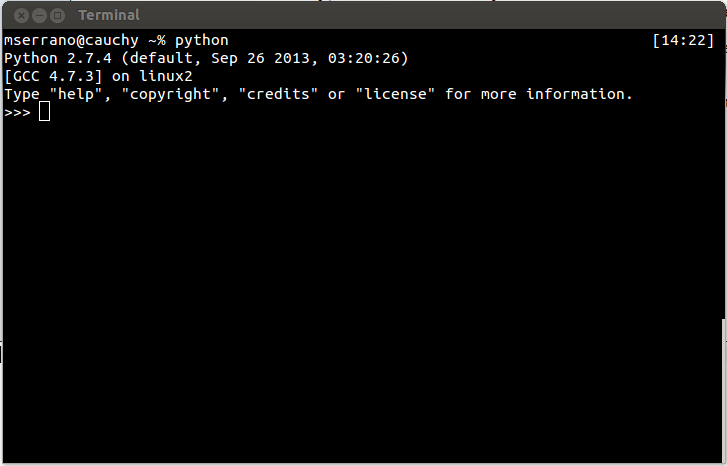
\includegraphics[height=6cm]{pic1.png}

\item Type \verb+exit()+ to exit out of Python. You now have Python and Pip installed!
\end{enumerate}
\subsection{Step 2 - Install Flask}
This step outlines how to install Flask using Pip, a package manager for Python libraries and utilities.
\begin{enumerate}
\item Open a terminal, or use an already open terminal.
\item Within the terminal, type the following command:
\begin{verbatim}
sudo pip install Flask
\end{verbatim}
You may be asked for your password. If you are, type it in. The characters you type for your password
will not display - but rest assured that they are being kept track of. You
may also be asked whether or not you  are sure. When that prompt appears, 
simply hit the Enter key to accept.
\item Open your favorite text editor, such as \verb+vim+ or \verb+emacs+. \pagebreak
\item Type the following text into your text editor:
\begin{verbatim}
from flask import Flask
app = Flask(__name__)
@app.route("/")
def hello():
    return "Hello world!"

app.run()
\end{verbatim}
\item Save the file as \verb+flask_test.py+ and close it.
\item Run the file by typing \verb+python flask_test.py+.
\item Open your web browser, and navigate to \verb+http://localhost:5000/+. You should see something like the following:

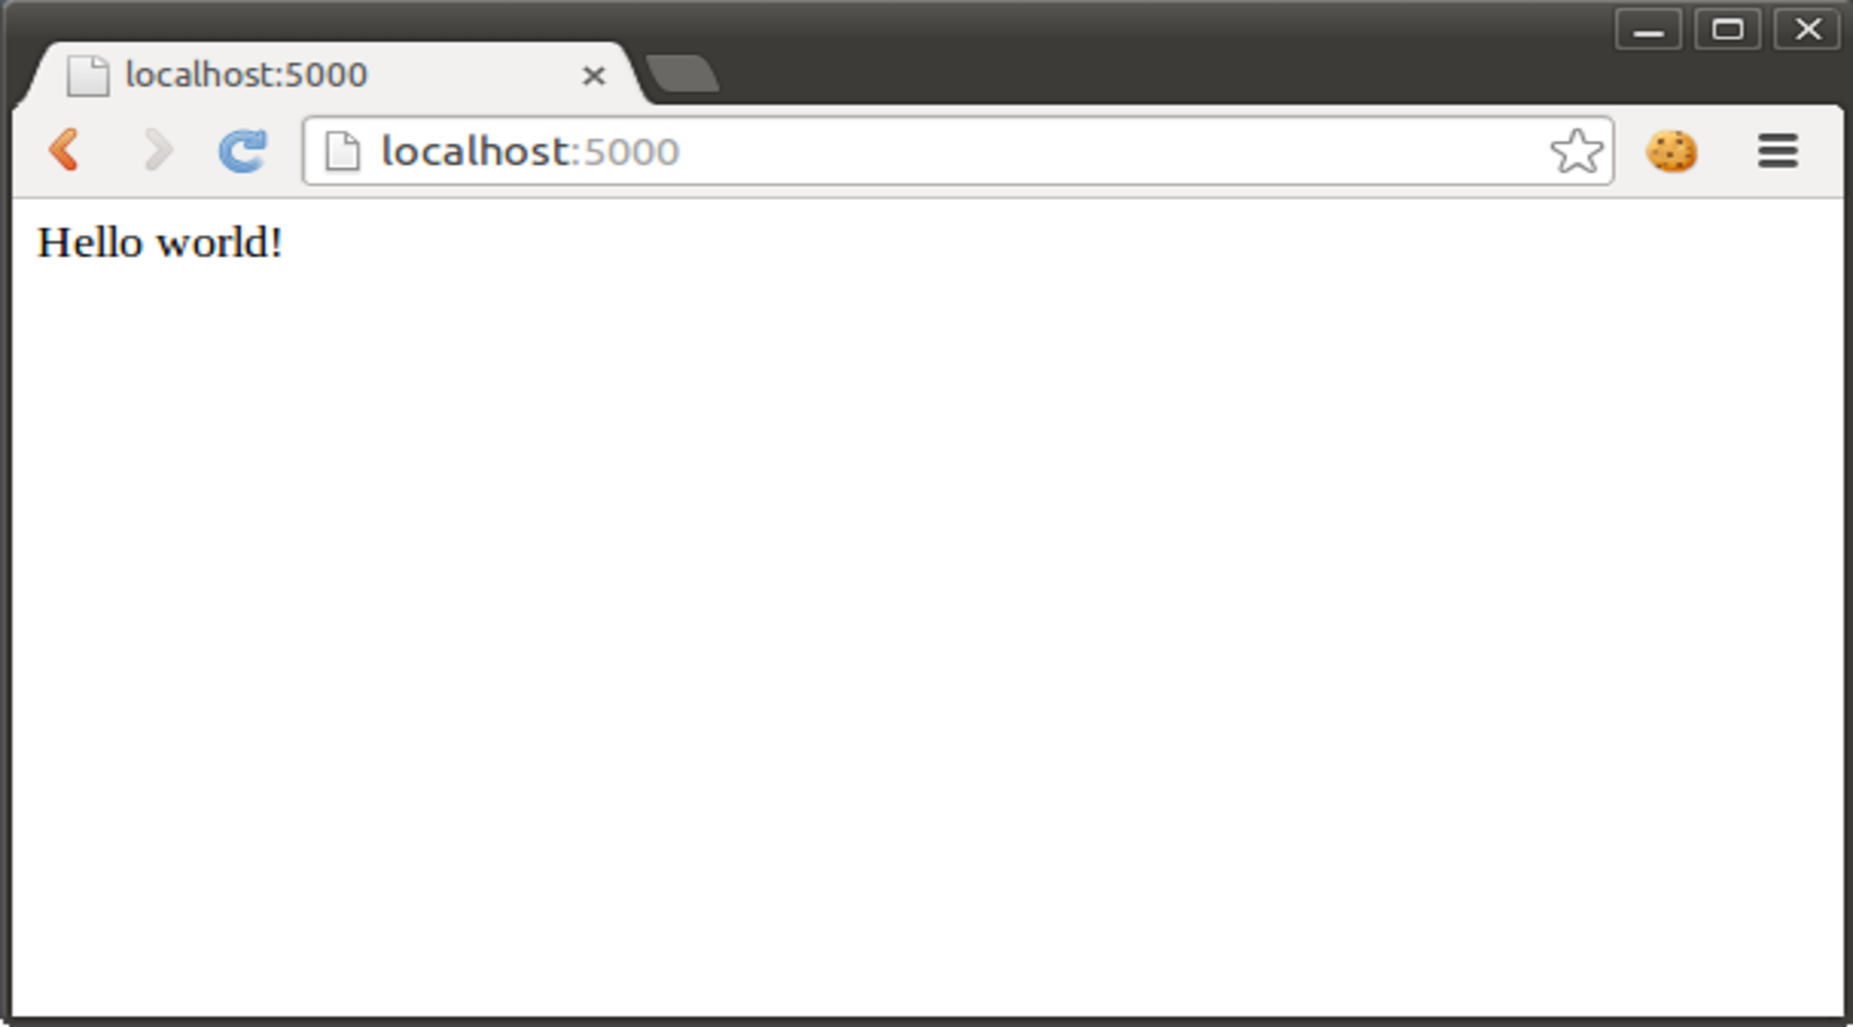
\includegraphics[height=6cm]{pic2.png}
\item Go back to your terminal, and hit Ctrl-C.
\item You now have Flask installed for development!
\end{enumerate}
\subsection{Step 3 - Install Apache}
This step outlines how to install Apache, a development-ready web server.
\begin{enumerate}
\item Open a terminal, or use an already open terminal.
\item Within the terminal, type the following command:
\begin{verbatim}
sudo apt-get install apache2 libapache2-mod-wsgi
sudo /etc/init.d/apache2 restart
\end{verbatim}
You may be asked for your password. If so, type it in. The characters you type for your password
will not display - but rest assured that they are being kept track of. You
may also be asked whether or not you are sure. When that prompt appears, simply hit the Enter key
to accept.
\pagebreak
\item Open a web browser, and navigate to \verb+http://localhost/+. You should see something like the following:


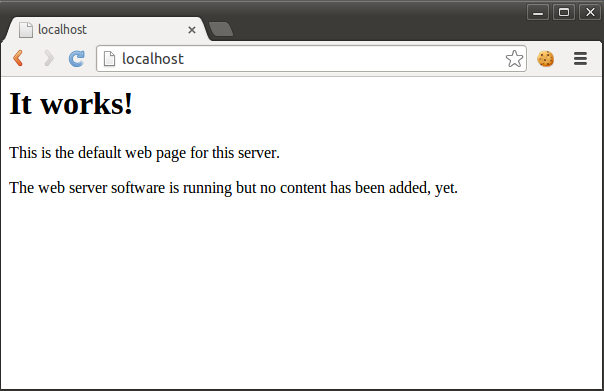
\includegraphics[height=6cm]{pic3.png}

\item Within your terminal, type the command \verb+sudo /etc/init.d/apache2 stop+.
\item You should now have Apache installed, though it will not yet be running.
\end{enumerate}
\subsection{Step 4 - Setup a Flask app in Apache}
This step outlines how to create a Flask app that Apache will run for you.
\begin{enumerate}
\item Open a terminal, or use an already open terminal.
\item Type \verb+sudo su+ into your terminal, and provide your password. Your terminal
now belongs to the \verb+root+ user - be very careful with the rest of your changes
from now on.
\item Type \verb+cd /var/www/+ into your terminal. Now, type \verb+mkdir app; cd app+.
\item Once you are safely in the \verb+app+ folder, your terminal should look like the following:

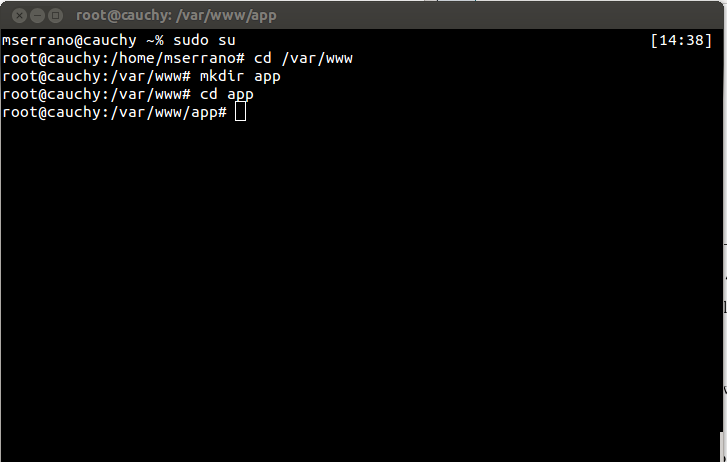
\includegraphics[height=6cm]{pic4.png}

\item Type \verb+touch application.wsgi+.
\item Open \verb+application.wsgi+ in your favorite editor, and type the following into it:
\begin{verbatim}
import sys
sys.path.append('/var/www/app')
from website import app as application
\end{verbatim}
\item Save and close the file.
\item Type \verb+touch website.py+.
\item Open \verb+website.py+ in  your favorite editor, and type the following into it:
\begin{verbatim}
from flask import Flask
app = Flask(__name__)

@app.route("/")
def hello():
    return "Hello world, from Apache!"
\end{verbatim}
\item Save and close the file.
\end{enumerate}
\subsection{Step 5 - Configure Apache to see the Flask App}
This step outlines how to inform Apache of how to run your Flask app.
\begin{enumerate}
\item Type \verb+cd /etc/apache2+ into your root terminal.
\item Open the file \verb+sites-available/default+ with your favorite editor, and
replace its contents with:
\begin{verbatim}
<VirtualHost *:80>
	ServerName localhost
    WSGIScriptAlias / /var/www/app/application.wsgi
    <Directory /var/www/app>
        Order deny,allow
        Allow from all
    </Directory>
</VirtualHost>
\end{verbatim}
\item Save and close the file.
\item Type \verb+/etc/init.d/apache2 restart+ into your terminal.
\item Open your web browser, and navigate to \verb+http://localhost/+. You should see something
like the following:

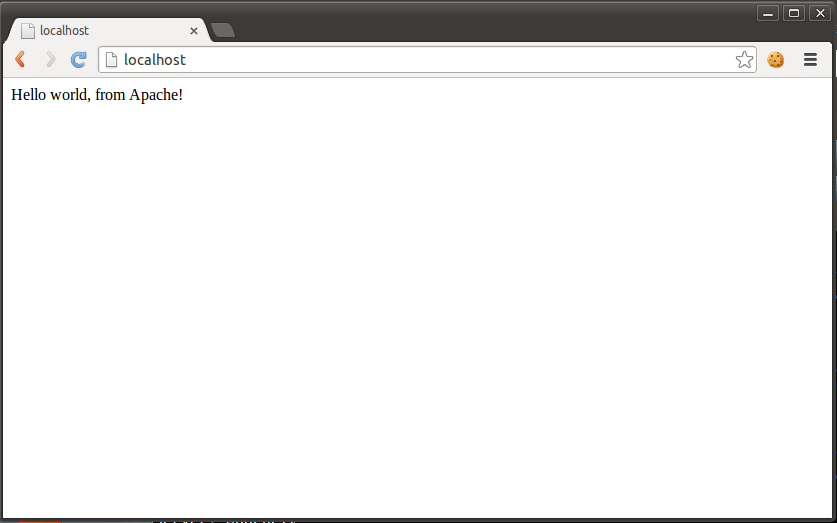
\includegraphics[height=6cm]{pic5.png}

\item Close your root terminal.
\item Congratulations! You now have Flask deployed in a production environment. When you make
changes, simply edit the file \verb+/var/www/app/website.py+, and type \verb+sudo /etc/init.d/apache2 restart+ to have the changes reflected by Apache.
\end{enumerate}
\end{document}